\documentclass{article}\usepackage[]{graphicx}\usepackage[]{color}
%% maxwidth is the original width if it is less than linewidth
%% otherwise use linewidth (to make sure the graphics do not exceed the margin)
\makeatletter
\def\maxwidth{ %
  \ifdim\Gin@nat@width>\linewidth
    \linewidth
  \else
    \Gin@nat@width
  \fi
}
\makeatother

\definecolor{fgcolor}{rgb}{0.345, 0.345, 0.345}
\newcommand{\hlnum}[1]{\textcolor[rgb]{0.686,0.059,0.569}{#1}}%
\newcommand{\hlstr}[1]{\textcolor[rgb]{0.192,0.494,0.8}{#1}}%
\newcommand{\hlcom}[1]{\textcolor[rgb]{0.678,0.584,0.686}{\textit{#1}}}%
\newcommand{\hlopt}[1]{\textcolor[rgb]{0,0,0}{#1}}%
\newcommand{\hlstd}[1]{\textcolor[rgb]{0.345,0.345,0.345}{#1}}%
\newcommand{\hlkwa}[1]{\textcolor[rgb]{0.161,0.373,0.58}{\textbf{#1}}}%
\newcommand{\hlkwb}[1]{\textcolor[rgb]{0.69,0.353,0.396}{#1}}%
\newcommand{\hlkwc}[1]{\textcolor[rgb]{0.333,0.667,0.333}{#1}}%
\newcommand{\hlkwd}[1]{\textcolor[rgb]{0.737,0.353,0.396}{\textbf{#1}}}%

\usepackage{framed}
\makeatletter
\newenvironment{kframe}{%
 \def\at@end@of@kframe{}%
 \ifinner\ifhmode%
  \def\at@end@of@kframe{\end{minipage}}%
  \begin{minipage}{\columnwidth}%
 \fi\fi%
 \def\FrameCommand##1{\hskip\@totalleftmargin \hskip-\fboxsep
 \colorbox{shadecolor}{##1}\hskip-\fboxsep
     % There is no \\@totalrightmargin, so:
     \hskip-\linewidth \hskip-\@totalleftmargin \hskip\columnwidth}%
 \MakeFramed {\advance\hsize-\width
   \@totalleftmargin\z@ \linewidth\hsize
   \@setminipage}}%
 {\par\unskip\endMakeFramed%
 \at@end@of@kframe}
\makeatother

\definecolor{shadecolor}{rgb}{.97, .97, .97}
\definecolor{messagecolor}{rgb}{0, 0, 0}
\definecolor{warningcolor}{rgb}{1, 0, 1}
\definecolor{errorcolor}{rgb}{1, 0, 0}
\newenvironment{knitrout}{}{} % an empty environment to be redefined in TeX

\usepackage{alltt}

\title{A Dynamic Document with R and \LaTeX}
\author{Matthias Bannert}

%%% MAYBE SHOW SOME REAL PAPERS, pdf of papers !
\IfFileExists{upquote.sty}{\usepackage{upquote}}{}
\begin{document}
\maketitle

\newpage

\section{Some Text}
Lorem ipsum dolor sit amet, consectetur adipiscing elit. Proin velit erat, vestibulum non posuere sit amet, ornare sit amet turpis. Duis congue, risus et malesuada sollicitudin, ante sapien vulputate eros, vitae accumsan quam mauris vel sapien. Etiam velit massa, rhoncus et rutrum sit amet, iaculis non nibh. Donec vitae lectus odio. Ut ullamcorper quis enim non hendrerit. In turpis dolor, consectetur et massa eget, porta laoreet orci. Maecenas fringilla ipsum eget eros suscipit volutpat. Sed in odio orci. Curabitur leo nisl, pharetra non laoreet nec, viverra eget tortor. Vivamus vestibulum, risus vitae varius mattis, velit quam dictum urna, vel sagittis dui augue auctor lacus. Nam non magna dolor.

\section{First Section}

Let's use the example of the Breusch Pagan test we have seen before... 

\begin{knitrout}
\definecolor{shadecolor}{rgb}{0.969, 0.969, 0.969}\color{fgcolor}
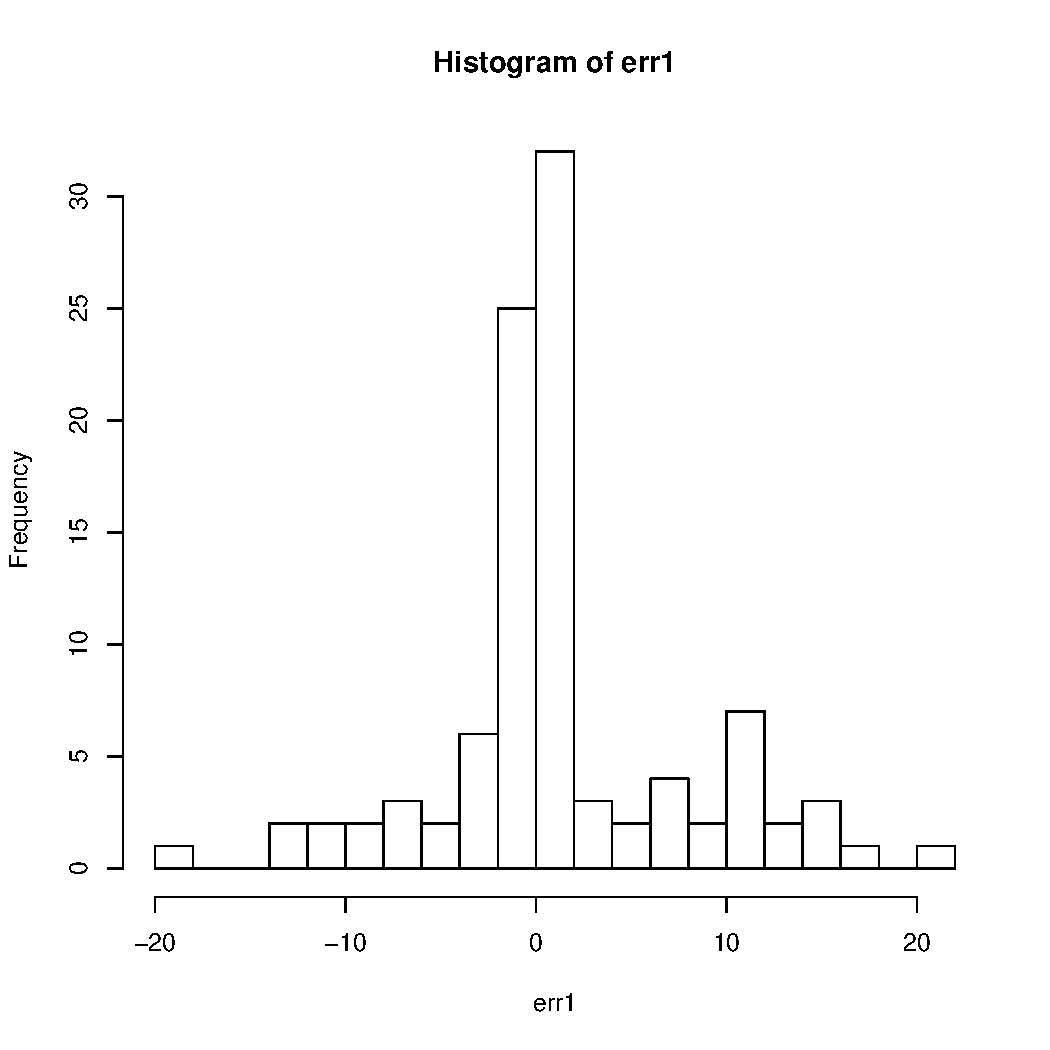
\includegraphics[width=\maxwidth]{figure/first-1} 

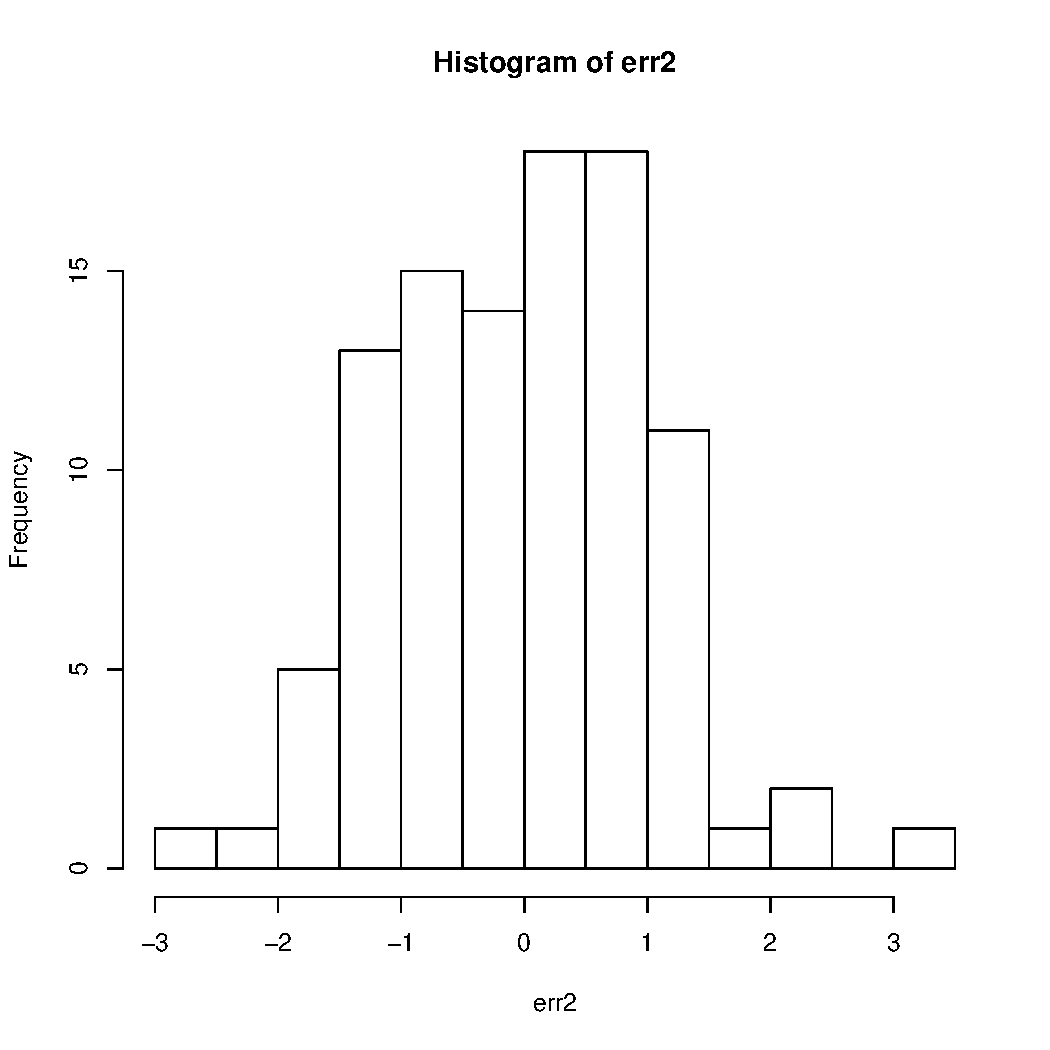
\includegraphics[width=\maxwidth]{figure/first-2} 

\end{knitrout}

The test results are also created dynamically. 

\begin{knitrout}
\definecolor{shadecolor}{rgb}{0.969, 0.969, 0.969}\color{fgcolor}\begin{kframe}
\begin{verbatim}
## 
## 	studentized Breusch-Pagan test
## 
## data:  y1 ~ x
## BP = 27.1634, df = 1, p-value = 1.87e-07
## 
## 	studentized Breusch-Pagan test
## 
## data:  y2 ~ x
## BP = 0.2779, df = 1, p-value = 0.5981
\end{verbatim}
\end{kframe}
\end{knitrout}














\end{document}
